% Chapter 3: Methodology

This chapter describes the methods and approaches used in the experiments. This includes dataset preparation, models, loss functions, etc.

\section{Overview of Approach}
An overall description of the approach to tackling the long-tailed dataset problem, including an explanation of the strategy, 
such as balancing techniques and model selection.

\section{Dataset Preparation and Specifications}
The first step is to prepare the data for training and testing. In order to generate training, validation, and test datasets that resemble the datasets used for the empirical studies in \textit{Deep Long-Tailed Learning: A Survey} \cite{zhang2023deep}, their dataset are investigated: The GitHub repository \cite{VanintLT} for the paper \textit{Deep Long-Tailed Learning: A Survey} was downloaded and an environment was set up on the Jupyter Hub on the Freja node on the ece cluster. The \texttt{.txt} files with the data from ImageNet-LT (\texttt{ImageNet\_LT\_train.txt}, \texttt{ImageNet\_LT\_val.txt}, \texttt{ImageNet\_LT\_test.txt}) are shown on figures \ref{fig:IN-train}, \ref{fig:IN-val}, and \ref{fig:IN-test}, respectively. TODO: Describe the plots and what they mean for my data preparation. 

\begin{figure}[h!]
    \centering
    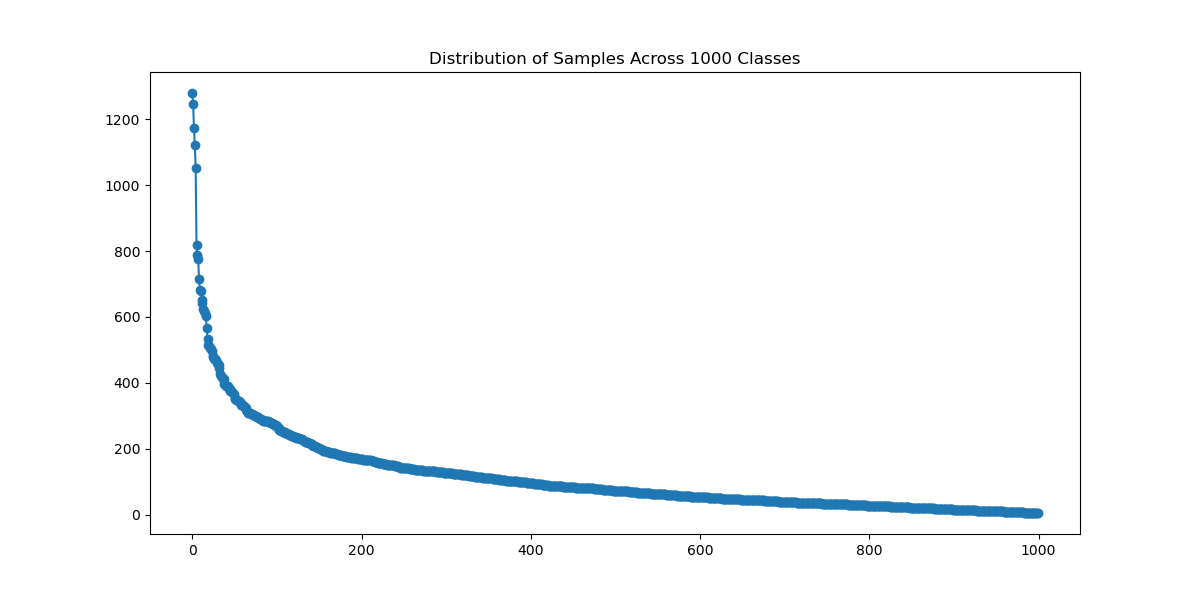
\includegraphics[width=0.9\textwidth]{Images/Plots/class_distribution_train.png}
    \caption{The class distribution of the training images for the ImageNet-LT dataset shows a long-tailed distribution.}
    \label{fig:IN-train}
\end{figure}

\begin{figure}[h!]
    \centering
    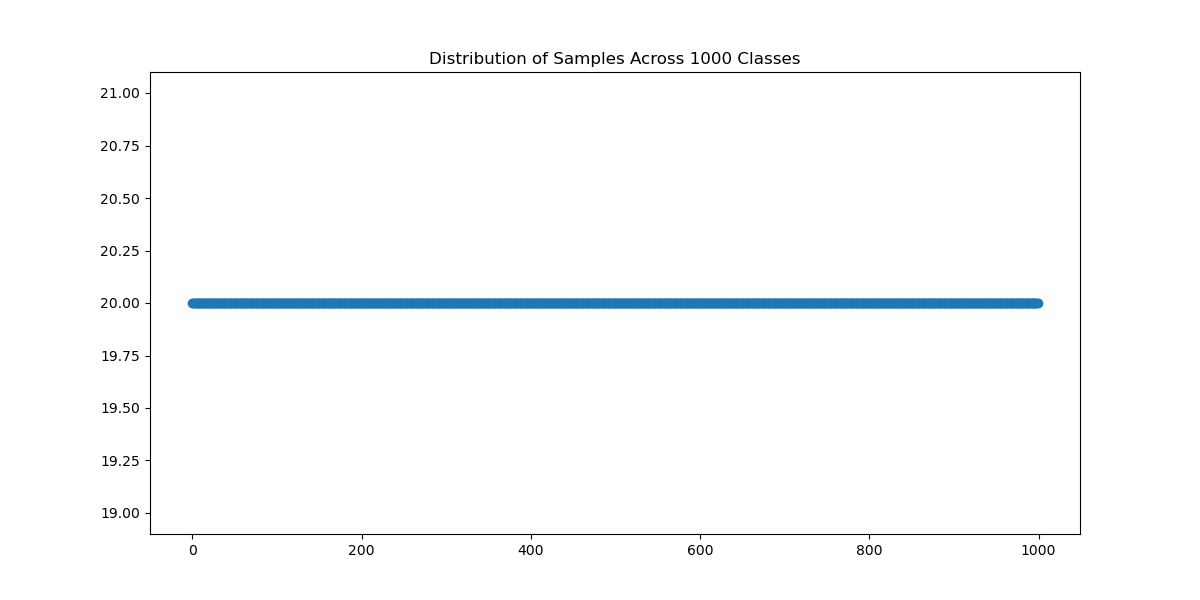
\includegraphics[width=0.9\textwidth]{Images/Plots/class_distribution_val.png}
    \caption{The class distribution of the validation images for the ImageNet-LT dataset shows that there are 20 samples of each class.}
    \label{fig:IN-val}
\end{figure}

\begin{figure}[h!]
    \centering
    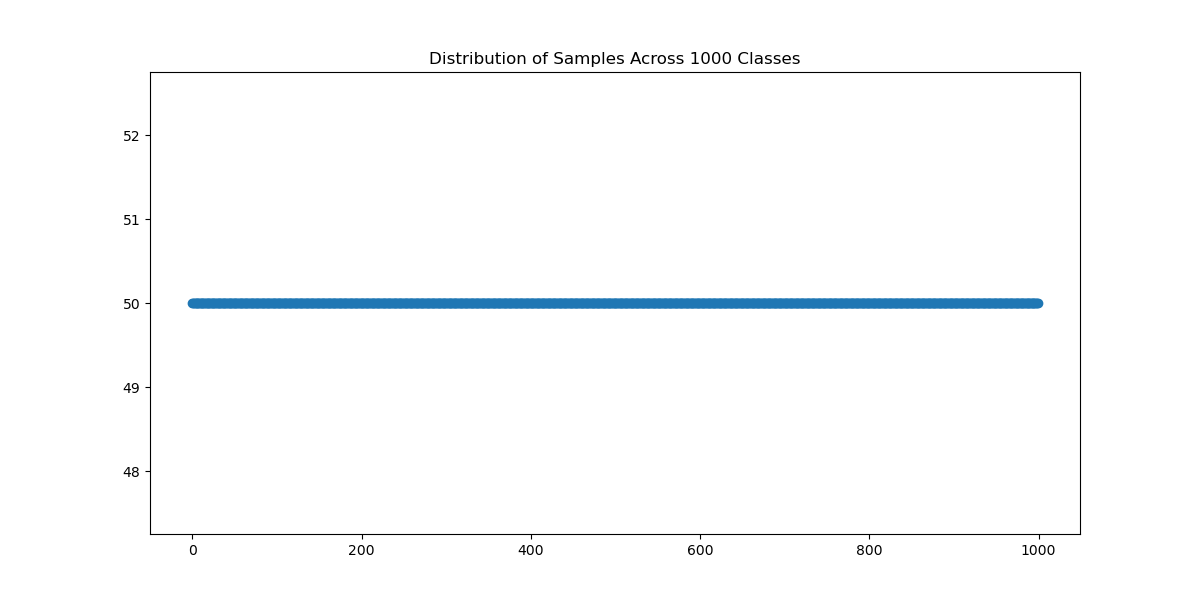
\includegraphics[width=0.9\textwidth]{Images/Plots/class_distribution_test.png}
    \caption{The class distribution of the test images for the ImageNet-LT dataset shows that there are 50 samples of each class.}
    \label{fig:IN-test}
\end{figure}

Following the dataset structure used in \textit{Deep Long-Tailed Learning: A Survey}, the CIFAR100 dataset was modified to create a long-tailed training set and a balanced test set. Key details include:

\begin{itemize}
    \item Dataset characteristics: Number of classes, imbalance ratio, and train-test splits.
    \item Preprocessing steps: Resizing, normalization, and augmentation techniques.
    \item Handling imbalance: Techniques like re-sampling and augmentation to address the long-tailed distribution.
\end{itemize}

\section{Model and Algorithm Selection}
Description of the model architectures chosen, and why they are appropriate for long-tailed learning.
Discussion of the strengths and limitations of these models in addressing the challenges posed by imbalanced data.

\subsection{Long-tailed Learning Techniques}
Description of the specific methods used to address class imbalance, such as data sampling, class re-weighting, etc. 
Justification for selecting these techniques, potentially referencing prior research (from Deep Long-Tailed Learning: A Survey by Zhang et al.).

% \subsection{Arguments}
% The reason the focus has been on class-sensistive learning form the re-balancing methods, is that re-sampling comes with challenges regarding knowing the dataset prior to training the model. we want to find the best method for classifying the moth dataset, on which we have no ability to test. TODO: this might not be the case. 

\subsubsection{Loss Functions}
Explanation of the different loss functions explored, such as cross-entropy, focal loss, LDAM loss, etc., and their relevance for long-tailed learning.
Rationale for each loss function's inclusion, focusing on its expected benefits for imbalanced classes and how it addresses the bias toward majority classes.



\section{Evaluation Metrics}
Justification for the metrics and evaluation approach, such as using weighted or macro F1 scores.
Explanation of how the performance is assessed across different class groups to capture the model’s performance on minority classes.

\section{Reproducibility}
Steps taken to ensure reproducibility of experiments:
\begin{itemize}
    \item Use of random seed initialization.
    \item Documentation of dataset versions and codebase.
    \item Availability of scripts for dataset preparation and model training.
\end{itemize}

\section{Implementation Details}
Technical explanations of any unique or customized methods implemented in code, for example the custom dataset.


